I aktiv modus er strømmen gjennom collector
proporsjonal med strømmen gjennom base.
Forstørrelsen er gitt ved $\beta$.
$$I_C = \beta \cdot I_B$$
Hvor strømforsterkningen $\beta$ er mellom 50 og 300.
\\\\
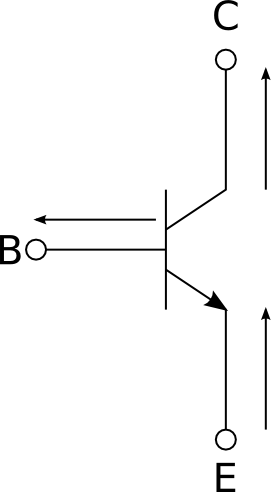
\includegraphics[width=0.25\textwidth]{./img/npn-strom}
\\\\
Strømmen gjennom emitter er lik
summen av strømmen gjenno base og collector.
$$I_E = I_B + I_C$$
